\scanpage{68}

est déterminé par la connaissance de
\[
K_0:A_0^0=A_0\longrightarrow M
\]
et $K_0$ \unsure{quelconque}, un $(K_n)$ \unsure{'|$\exists$} ssi
\[
K_0\bigl(\partial_1(\operatorname{Ker}(A_1^0\xrightarrow{d}A_1^1))\bigr)=0
\]
(donc il y a un syst. d'intégrale de Stokes-DeRham ``universel'' à valeurs dans
\[
A_0/\partial_1(\operatorname{Ker}(A_1^0\xrightarrow{d}A_1^1)),
\]
le cas le plus intéressant est celui où
\[
\partial_1(\operatorname{Ker}(A_1^0\overset{d}{\text{---}}A_1^1))=0,
\]
donc où le \unsure{choix universel|domaine universel} est pour $M=A_0$, ce qui sera le cas en particulier si on a
\[
\mathrm{c}')\quad H^0(A_1^*)\xleftrightarrow{\sim}\varepsilon^*(A_0^0)
\qquad(\text{où }\varepsilon:\Delta_1\longrightarrow\Delta_0\ldots)
\]
(ce qui est une variante de c) pour $n=1$).

\margin{ou $H^0(A_1^*)=\varepsilon^*(Z_0^0)$ \unsure{dans le cas où l'on présume a), en général}}
\figure{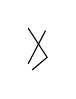
\begin{tikzpicture}\draw (0,.45)--(.24,.08)--(.05,-.08);\draw (0,0)--(.22,.42);\end{tikzpicture}}

Sous ces conditions, on sait donc qu'il existe un \uline{unique} hom de complexes de modules $1/2$ simpliciaux
\[
A_*^*\longrightarrow C_{*M}^*.
\]
qui sur $A_0^0=A_0$ coïncide avec
\[
K_0:A_0^0\longrightarrow \unsure{C|R}_{0M}^0=M
\]
(donc l'identité; le \unsure{cas|syst.} prototype).

On peut noter qu'en fait cet hom est même à valeurs dans $C_{*M}^{*!}$ (les cochaines non dégénérées), i.e. on a en fait
\[
A_*^*\longrightarrow C_{*M}^{*!}\simeq
\Lambda^{*+1}\unsure{\Phi|Q}_{*k}\otimes_k M
\]
en se rappelant que
\[
C_{*M}^{n!}=
\bigcap_{\unsure{\sigma:\Delta_n\twoheadrightarrow\Delta_m,\ m<n}}
\operatorname{Ker}(C_{*M}^{n}\xrightarrow{\sigma^*}C_{*M}^{m})
\]
\margin{67}
